%  Mikroprozessor Praktikum Protokolle
%
%  Sebastian Raitza, Nico von Geyso 2010
%
\documentclass[11pt,german]{scrartcl}

% See geometry.pdf to learn the layout options.
\usepackage[top=2.5cm,bottom=2.5cm,left=2.5cm,right=2.5cm]{geometry}
\geometry{a4paper}

% To begin paragraphs with an empty line
\usepackage[parfill]{parskip}

% Use utf-8 encoding for foreign characters
\usepackage[utf8]{inputenc}
\usepackage[T1]{fontenc}

\usepackage{ngerman}
\RequirePackage[ngerman=ngerman-x-latest]{hyphsubst}

% Running Headers and footers
\usepackage{fancyhdr}
\pagestyle{fancyplain}

% More symbols
\usepackage{amsmath}
\usepackage{amssymb}
%\usepackage{latexsym}

% URLs and Links
\usepackage{url}
\usepackage{makeidx}
\usepackage[colorlinks=true, linkcolor=blue, urlcolor=blue]{hyperref}

% Surround parts of graphics with box
\usepackage{boxedminipage}

% Package for including code in the document
\usepackage{listings}
\usepackage{color}
\usepackage{moreverb}
\usepackage{courier}


% This is now the recommended way for checking for PDFLaTeX:
\usepackage{ifpdf}

\ifpdf
\usepackage[pdftex]{graphicx}
\else
\usepackage{graphicx}
\fi

\ifpdf
\DeclareGraphicsExtensions{.pdf, .jpg, .tif}
\else
\DeclareGraphicsExtensions{.eps, .jpg}
\fi

% Create hyperlinks
\usepackage{hyperref}
\hypersetup{
    colorlinks=false,       % false: boxed links; true: colored links
    linkcolor=red,          % color of internal links
    citecolor=green,        % color of links to bibliography
    filecolor=magenta,      % color of file links
    urlcolor=cyan           % color of external links
}

\makeindex

\title{Mikroprozessor Praktikum\\Protokolle 1-22}
\author{Sebastian Raitza, Nico von Geyso}

% Activate to display a given date or no date
\date{23. Februar 2011}

%%%%%%%%%%%%%%%%%%%%%%%%%%%%%%%%%%%%%%%%%%%%%%%%%%%%%%%%%%%%%%%%%%

\renewcommand{\labelenumi}{\alph{enumi})}
\renewcommand{\labelenumii}{$\bullet$}

% define a macro ausgabe which takes as argument
% your ausgabe.txt file’s name
\newcommand{\ausgabe}[1] {\hrule\small\verbatiminput{#1}\normalsize\hrule}

\definecolor{light-gray}{gray}{0.95}

\lstset{
  language=C,               % choose the language of the code
  basicstyle=\ttfamily\scriptsize,   % size of fonts used for the code
  numbers=left,             % where to put the line-numbers
  numberstyle=\scriptsize,        % size of fonts for used line-numbers
  stepnumber=1,             % step between line-numbers
  numbersep=5pt,            % how far the line-numbers are from the code
  backgroundcolor=\color{white},  % background color, add \usepackage{color}
  showspaces=false,         % show spaces adding particular underscores
  showstringspaces=false,   % underline spaces within strings
  showtabs=false,           % show tabs within strings adding particular underscores
  frame=single,             % adds a frame around the code
  tabsize=4,                % sets default tabsize to 2 spaces
  captionpos=b,             % sets the caption-position to bottom
  breaklines=true,          % sets automatic line breaking
  breakatwhitespace=false,  % sets if automatic breaks should only happen at whitespace
  escapeinside={\%*}{*)},   % if you want to add a comment within your code
  frameround=tttt,
  extendedchars=true,
  literate=%
    {Ö}{{\"O}}1
    {Ä}{{\"A}}1
    {Ü}{{\"U}}1
    {ß}{{\ss}}2
    {ü}{{\"u}}1
    {ä}{{\"a}}1
    {ö}{{\"o}}1
    {°}{{}}0
}

\begin{document}

\maketitle

%\tableofcontents

\section{Modulbeschreibung des Mikroprozessor-Praktikums}
%\addcontentsline{toc}{section}{Modulbeschreibung des
%Mikroprozessor-Praktikums}

$\frac{5}{5}$

Die überwältigende Mehrheit zukünftiger Computersysteme wird durch miteinander kommunizierende, eingebettete Systeme geprägt sein.
Diese finden sich in Maschinensteuerungen, Haushaltsgeräten, Kraftfahrzeugen, Flugzeugen, intelligenten Gebäuden etc. und
werden zukünftig immer mehr in Netze wie dem Internet eingebunden sein.
Das Praktikum wird auf die Architektur eingebetteter Systeme eingehen und die Unterschiede zu traditionellen PC-Architekturen
(z.B. Echtzeitfähigkeit, Interaktion mit der Umgebung) anhand praktischer Beispiele aufzeigen.
Das Praktikum basiert auf einem MSP430 Mikrocontrollersystem.
Schwerpunkte des in einzelne Versuche gegliederten Praktikums sind:
\begin{itemize}
    \item Registerstrukturen
    \item Speicherorganisation
    \item hardwarenahe Assembler- und Hochsprachenprogrammierung
    \item I/O-System- und Timer-Programmierung
    \item Interrupt-System
    \item Watchdog-Logik
    \item Analogschnittstellen
    \item Bussystemanbindung von Komponenten
    \item Kommunikation (seriell, CAN-Bus, Ethernet, Funk und USB)
    \item Ansteuerung von Modellen und Nutzung unterschiedlichster Sensorik.
\end{itemize}


\section{Entwicklungsboard MSB430H}
%\addcontentsline{toc}{section}{Entwicklungsboard MSB430H}
Auf dem zum entwickelten Board handelt es sich um das Entwicklungsboard MSB430H.
Der hier verwendete Mikrocontroller ist ein MSP430F1612 von Texas Instrument.
Dieser verfügt neben einem universellen Clock-System unter anderem über 55 kByte Flash, 5kByte Ram, USART und einem Watchdog.
Das Board ist zusätzlich mit einem 868MHz Transceiver (CC1100),
sowie einem Luftfeuchtigkeits- und Temperatursensor (SHT11), einem 3D-Beschleunigungssensor (MMA7260Q)
und einer SD-Karte ausgestattet.

%%%%%%%%%%%%%%%%%%%%%%%%%%%%%%%%%%%%%%%%%%%%%%%%%%%%%%%%%%%%%%%%%%

%\clearpage
\section
{\href{http://cst.mi.fu-berlin.de/intern/19606-P-MPP/Aufgaben/040100.html}
{I/O Portleitungen}}
%\addcontentsline{toc}{section}{I/O Portleitungen}

Ein Kennzeichen von Mikrocontrollern sind ihre I/O-Portleitungen.
Auch bekannt unter dem Namen \textit{General Purpose Input/Output}.
Diese Pins können als Eingang um digitale Signale zu lesen fungieren
oder als Ausgang um andere Geräte zu kontrollieren oder mit ihnen zu kommunizieren.

Die Konfiguration dieser kann mittels Software programmiert werden
und überlässt so dem Entwickler große Freiheiten.
Bei manchen Mikrocontrollern können einige I/O-Ports des Weiteren als Interruptquellen definiert werden.

Meist werden die I/O-Pins in unterschiedliche Ports gruppiert.
Ein Port hat meistens acht I/O-Pins.

Der von uns verwendete MSP430F1612 verfügt über sechs I/O-Ports mit jeweils acht Bit Breite.

\subsection
{\href{http://cst.mi.fu-berlin.de/intern/19606-P-MPP/Aufgaben/040101.html}
{Aufgabe 1: Portleitung als Output}}

Jeder Pin kann über die 8-Bit Register PxDIR, PxOUT und PxIN konfiguriert beziehungsweise ausgelesen werden.
X ist dabei ein Wert zwischen 0 und 5 – stehend für den jeweiligen Port.

Mittels dem i-ten Bit des PxDIR-Registers wird der $i$-te Pin des Ports $x$ als Eingang oder Ausgang konfiguriert.
Je nachdem kann im PxIN-Register der Wert gelesen bzw. im PxOUT-Register geschrieben werden.

Die Pins selber können nur zwei Zustände annehmen: HIGH (logisch Eins) und LOW (logisch Null).
\subsubsection*{Erläuterung von Befehlen}
\lstinputlisting[linerange=29-41,firstnumber=29,caption=aufgabe01.c]
{../MPP_WS1011/aufgaben/aufgabe01.c}

\subsubsection*{Ampelschaltung}

Um eine Ampelschaltung zu realisieren wird in festeinprogrammierten Zeitabständen die jeweilige LED-Kombination eingeschaltet.
\lstinputlisting[linerange=46-70,firstnumber=46,caption=aufgabe01.c]
{../MPP_WS1011/aufgaben/aufgabe01.c}

\subsection*{Aufgabe 2: Portleitung als Input}

\subsubsection*{Erklärung der Befehlszeilen}
\lstinputlisting[linerange=16-29,firstnumber=16,caption=aufgabe02.c]
{../MPP_WS1011/aufgaben/aufgabe02.c}

\subsubsection*{Tastenprogramm}
\lstinputlisting[linerange=43-70,firstnumber=43,caption=aufgabe02.c]
{../MPP_WS1011/aufgaben/aufgabe02.c}

\subsection*{
\href{http://cst.mi.fu-berlin.de/intern/19606-P-MPP/Aufgaben/040103.html}
{Aufgabe 3: Ampelsteuerung}}

\lstinputlisting[linerange=17-83,firstnumber=17,caption=aufgabe03.c]
{../MPP_WS1011/aufgaben/aufgabe03.c}


\subsection
{\href{http://cst.mi.fu-berlin.de/intern/19606-P-MPP/Aufgaben/040104.html}
{Aufgabe 4: Tastaturabfrage}}
Je nachdem welche Taste gedrückt wird der interne Zähle in- bzw. dekrementiert oder zurückgesetzt. 
Für die binäre Darstellung wird mittels einfacher booleschen Und-Operation und Schiebeoperation das jeweilige Bit ermittelt und dann die dazugehörige LED umgeschaltet.
\lstinputlisting[linerange=17-53,firstnumber=17,caption=aufgabe04.c]
{../MPP_WS1011/aufgaben/aufgabe04.c}




%%%%%%%%%%%%%%%%%%%%%%%%%%%%%%%%%%%%%%%%%%%%%%%%%%%%%%%%%%%%%%%%%%

\clearpage
\section
{\href{http://cst.mi.fu-berlin.de/intern/19606-P-MPP/Aufgaben/040200.html}
{Clock System}}
%\addcontentsline{toc}{section}{Clock System}

\subsection*
{\href{http://cst.mi.fu-berlin.de/intern/19606-P-MPP/Aufgaben/040201.html}
{Aufgabe 5: Frequenzmessung der Taktquellen}}

\subsubsection*{Vorbereitung}
\begin{lstlisting}
void Aufgabe5() {
    P5SEL |= BIT4;    // P5 MCLK
}
\end{lstlisting}

\subsubsection*{Messwerte}
\paragraph{LFXT1CL} \texttt{(SELM = 11b)}
\begin{description}
    \item [LF-Mode] \texttt{(XTS = 0)}
        \begin{enumerate}
            \item minimal: 12,29kHz, DIVM=11b
            \item maximal: 32,769, DIVM=00
        \end{enumerate}

    \item [HF-Mode] \texttt{(XTS = 1)}
        \begin{enumerate}
            \item minimal: 636,5kHz, DIVM=11b
            \item maximal: 1,695 MHz, DIVM=00
        \end{enumerate}
\end{description}

\paragraph{XT2CL} \texttt{(SELM = 11b, XT2OFF=0)}
\begin{enumerate}
    \item minimal: 635 KHz, DIVM=11b
    \item maximal: 1,695 MHz, DIVM=00
\end{enumerate}

\paragraph{DCOCLK} \texttt{(SELM = 00b)}
\begin{enumerate}
    \item minimal: 393,2 kHz, DCO=000b, RSEL=000b, DIVM=11b, MOD = 00000b
    \item normal: 7,36 mHz, DCO=011b, RSEL=100b, DIVM=00b, MOD = 11101b
    \item maximal: 11,59Mhz, DCO=111b, RSEL=111b, DIVM=00b, MOD hat keinen Effekt
\end{enumerate}

\paragraph{Erläutern Sie, wie der externe Widerstand für den DCOCLK-Taktgenerator nutzbar gemacht wird?}
Durch setzten des DCOR-Bits im BCSCTL2-Bit-Feld kann der externe Widerstand nutzbar gemacht werden.

\paragraph{Welchen Einfluss hat der Widerstand auf den DCOCLK-Taktgenerator?}
Der Widerstand verringert den Einfluss der Temperatur auf die Zuverlässigkeit des Taktgenerators. RC-Glied wieder niederohmiger und somit werden die Flanken deutlicher, da der Kondensator sich wieder schnell aufladen kann.


\subsection
{\href{http://cst.mi.fu-berlin.de/intern/19606-P-MPP/Aufgaben/040202.html}
{Aufgabe 6: Stromverbrauch und Taktfrequenz}}

Folgende Tabelle zeigt die Abhängigkeit des Stromverbrauchs von der Taktfrequenz. Der DCO\-CLK-Taktgenerator wurde durch manuelle Modifikation der DCOCTL, BCSCTL1 und BCSCTL2 Register im Debug-Modus des Code Composers auf Frequenzen im Bereich von 100kHz bis 10MHz eingestellt. Anschließend wurde jeweils der Stromverbrauch des Controllers im RUN-Modus am in Reihe geschalteten Digitalmultimeter gemessen. Die Tabelle enthält alle Messwerte mit den entsprechenden Bit-Settings der Clock-Register.

\begin{center}
\begin{tabular}{|r|c|c|c|c|c|}\hline
Frequenz in kHz	&	Strom in mA	&	RSEL	&	DCO	&	MOD	&	DIVM \\\hline

99,7	&	0,53	&	0	&	0	&	0	&	3 \\\hline
138,4	&	0,57	&	1	&	0	&	0	&	3 \\\hline
196,6	&	0,62	&	2	&	0	&	0	&	3 \\\hline
290,6	&	0,71	&	3	&	0	&	0	&	3 \\\hline
393,7	&	0,81	&	4	&	0	&	0	&	3 \\\hline
505,3	&	0,91	&	5	&	0	&	0	&	3 \\\hline
589,3	&	0,99	&	6	&	0	&	0	&	3 \\\hline
666,1	&	1,06	&	7	&	0	&	0	&	3 \\\hline
986,3	&	1,34	&	7	&	4	&	0	&	3 \\\hline
1.458,0	&	1,75	&	7	&	7	&	0	&	3 \\\hline
1.971,0	&	1,87	&	7	&	4	&	0	&	2 \\\hline
2.916,0	&	2,53	&	7	&	7	&	0	&	2 \\\hline
3.940,0	&	2,91	&	7	&	4	&	0	&	1 \\\hline
4.096,0	&	3,02	&	7	&	4	&	11	&	1 \\\hline
5.827,0	&	4,05	&	7	&	7	&	0	&	1 \\\hline
7.368,0	&	4,67	&	5	&	5	&	29	&	0 \\\hline
7.870,0	&	4,94	&	7	&	4	&	0	&	0 \\\hline
11.612,0	&	6,88	&	7	&	7	&	0	&	0 \\\hline

\end{tabular}
\end{center}

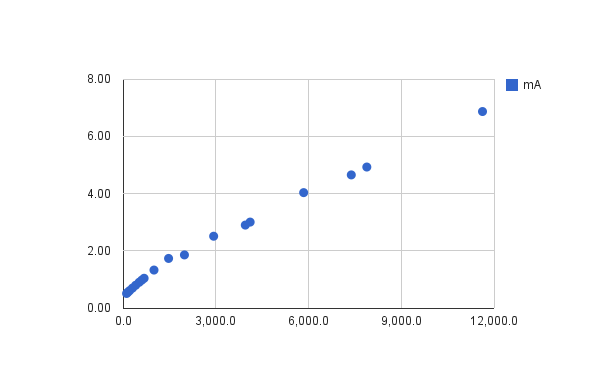
\includegraphics[width=\textwidth]{aufgaben/06/chart_2.png}

Das Diagramm zeigt den Stromverbrauch (vertikal) im Verhältnis zur Taktfrequenz (horizontal) der MCLK an Hand obiger Messwerte. Der Stromverbrauch stieg bei unseren Messungen grob proportional zur Taktfrequenz.


\subsection*{Aufgabe 7: Dynamische Taktfrequenzumschaltung}
\subsubsection*{Quelltext}

\lstinputlisting[linerange=10-21,firstnumber=10,caption=aufgabe07.c]
{../MPP_WS1011/aufgaben/aufgabe07.c}

\begin{lstlisting}[caption=Macros]
#define RSEL_RESET      (BCSCTL1 &= ~(RSEL0 | RSEL1 | RSEL2))
#define DCO_RESET       (DCOCTL &= ~(DCO0 | DCO1 | DCO2))
#define MOD_RESET       (DCOCTL  &= ~(MOD0 | MOD1 | MOD2 | MOD3 | MOD4))
#define DIVM_RESET      (BCSCTL2 &= ~(DIVM0 | DIVM1))
\end{lstlisting}

\lstinputlisting[linerange=57-95,firstnumber=57,caption=interrupts\_a07.c]
{../MPP_WS1011/aufgaben/interrupts_a07.c}


\subsection
{\href{http://cst.mi.fu-berlin.de/intern/19606-P-MPP/Aufgaben/040204.html}
{Aufgabe 8: Abarbeitungszeit eines Befehls}}

Mit Hilfe eines digitalen Taktzählers wird die Zeit zwischen unterschiedlichen Spannungswerten am Port \texttt{P5OUT} gemessen.
\subsubsection*{Messungen}
\begin{itemize}
    \item bei steigendender Flanke: $0,7 \mu s$
    \item bei fallender Flanke: $0,9 \mu s$
\end{itemize}
Bei steigender Flanke wird die Dauer von zwei \texttt{XOR}-Instruktionen gemessen.
Währenddessen bei fallender Flanke alle Befehle vom zweiten \texttt{XOR} bis zum erneuten Schleifeneintritt und der ersten \texttt{XOR}-Instruktionen gemessen werden. Dies beinhaltet einen weiteren \texttt{JMP}-Befehl und dauert somit länger.
\subsubsection*{Quelltext}

\lstinputlisting[linerange=10-20,firstnumber=10,caption=aufgabe08.c]
{../MPP_WS1011/aufgaben/aufgabe08.c}


%%%%%%%%%%%%%%%%%%%%%%%%%%%%%%%%%%%%%%%%%%%%%%%%%%%%%%%%%%%%%%%%%%

\clearpage
\section
{\href{http://cst.mi.fu-berlin.de/intern/19606-P-MPP/Aufgaben/040300.html}
{Watchdog}}
%\addcontentsline{toc}{section}{Watchdog}

\subsection*
{\href{http://cst.mi.fu-berlin.de/intern/19606-P-MPP/Aufgaben/040301.html}
{Aufgabe 9: Nutzung des Watchdog}}

\subsubsection*{Vorbereitung}

Kapitel 10 des \emph{User Guide}s beschreibt Funktionsweise des
WDT-Moduls und die Register zu dessen Ansteuerung. Für diese Aufgabe
sind folgende Bits des Kontrollregisters WDTCTL relevant:

\begin{description}
    \item [WDTPW]    Passwortschutz (mehr in Aufgabe 11)
    \item [WDTHOLD]  Der User-Guide empfielt das WDT-Modul vor einem
Intervallwechsel anzuhalten
    \item [WDTCNTCL] Setzt den Timer-Zähler auf
0 zurück \item [WDTSSEL]  Auswahl des Taktquelle (0 SMCLK, 1 ACLK)
    \item [WDTISx]   2 Bits selektieren den Teiler für die Taktquelle (0 für
$/32768$) \end{description}

\subsubsection*{Programm}

Ohne Programmierung der Taktquelle ist der Watchdog-Counter nach dem
Einschalten auf ein $32 ms$ Intervall initialisiert. Die LED würde nie
eingeschaltet.

Die ACLK-Taktquelle des \emph{Basic Clock Moduls} wird auf den Vorteiler
$/8$ programmiert ($4096 Hz$) und für den Watchdog-Timer ausgewählt. Das
Watchdog-Interval wird nach $32768 / 4096 Hz = 8 s$ erreicht, d.h. die
LED wird bei 0,5 Sek. Schaltzyklus 8-mal blinken, falls der
Watchdog-Counter nicht zurückgesetzt wurde.

Es ist nun völlig ausreichend den Watchdog pro Schleifendurchlauf (Dauer
$1 s$) über \texttt{WDTCNTCL} zurückzusetzen.

\subsubsection*{Quelltext}

\lstinputlisting[linerange=9-40,firstnumber=9,caption=aufgabe09.c]
{../MPP_WS1011/aufgaben/aufgabe09.c}

\subsection*{Aufgabe 10: Nutzung des Watchdog bei lokalen Problemen}

\subsubsection*{Programm}
Wird die äußere While-Schleife, in der der Watchdogzähler zurückgesetzt wird, zu lange
blockiert, ohne das dies im blockierendem Code beachtet wird, kann es zu unerwarteten
Resets durch den Watchdog kommen. Abhilfe ist hier natürlich in der innere Schleife, die
während eines Tastendrucks blockt, den Counter gesondert zu löschen.


\subsubsection*{Quellcode}
\lstinputlisting[linerange=9-45,firstnumber=9,caption=aufgabe10.c]
{../MPP_WS1011/aufgaben/aufgabe10.c}

\begin{comment}
Wie können Sie registrieren und speichern, wann und an welcher Programmstelle der Watchdog das System neu gestartet hat.

Skizzieren Sie einen Lösungsansatz. Als Hilfestellung hier folgende Stichwörter:

    NMI-Interrupt
    Stackpointer
    Programcounter
    Softwarereset
    INFOMEM
\end{comment}

\subsection*{Aufgabe 11: Reset per Software}

\lstinputlisting[linerange=9-21,firstnumber=9,caption=aufgabe11.c]
{../MPP_WS1011/aufgaben/aufgabe11.c}


%%%%%%%%%%%%%%%%%%%%%%%%%%%%%%%%%%%%%%%%%%%%%%%%%%%%%%%%%%%%%%%%%%

\clearpage
\section
{\href{http://cst.mi.fu-berlin.de/intern/19606-P-MPP/Aufgaben/040400.html}
{Interrupt}}
%\addcontentsline{toc}{section}{Interrupt}

Mittels Interrupt kann aufgrund von gewissen Ereignissen die normale Programmabarbeitung unterbrochen werden.
Dies ist hilfreich um auf Ereignisse an I/O-Ports oder Peripheriegeräten sofort reagieren zu können.

Folgende Interruptquellen sind auf dem MSP430F1612 verfügbar:

\begin{itemize}
    \item DA/Wandler und DMA
    \item I/O PORT 2
    \item USART1 Senden
    \item USART1 Empfangen
    \item I/O Port
    \item TIMER A
    \item A/D Wandler
    \item USART0 Senden
    \item USART1 Empfangen
    \item Watchdog Timer
    \item Comparator A
    \item Timer B
    \item NMI
    \item RESET
\end{itemize}

Um mit Interrupts arbeiten zu können müssen diese global aktiviert sein.
Hierfür ist das GIE-Bit im SR-Register zuständig.
Des Weiteren müssen für jede Interruptquelle, der Interrupt explizit erlaubt werden.

Wurde ein Interrupt ausgelöst, so wird die dafür geschriebene Interrupt Service Routine (ISR) abgearbeitet. Anzumerken sei, dass die ISR dafür zuständig ist, dass die jeweilige Interrupt-Flag wieder zurückgesetzt wird.
Wird dies nicht getan, so springt der Microcontroller sofort wieder in die ISR und es kommt zu einer Endlosschleife.

\subsection*{Aufgabe 12: Interrupt Quelle Taster}

\lstinputlisting[linerange=9-49,firstnumber=9,caption=aufgabe12.c]
{../MPP_WS1011/aufgaben/aufgabe12.c}

\lstinputlisting[linerange=55-76,firstnumber=55,caption=interrupts\_a12.c]
{../MPP_WS1011/aufgaben/interrupts_a12.c}

\subsection
{\href{http://cst.mi.fu-berlin.de/intern/19606-P-MPP/Aufgaben/040402.html}
{Aufgabe 13: Die Totmannschaltung mit Interrupt und Watchdog}}

\lstinputlisting[caption=aufgabe13.h]
{../MPP_WS1011/aufgaben/aufgabe13.h}

\lstinputlisting[linerange=10-77,firstnumber=21,caption=aufgabe13.c]
{../MPP_WS1011/aufgaben/aufgabe13.c}

\lstinputlisting[caption=interrupts\_a13.c]
{../MPP_WS1011/aufgaben/interrupts_a13.c}


%%%%%%%%%%%%%%%%%%%%%%%%%%%%%%%%%%%%%%%%%%%%%%%%%%%%%%%%%%%%%%%%%%

\clearpage
\section
{\href{http://cst.mi.fu-berlin.de/intern/19606-P-MPP/Aufgaben/040500.html}
{LPM-Modi}}
%\addcontentsline{toc}{section}{LPM-Modi}

Viele meist batteriebetriebene Mikrocontroller besitzen so genannte \emph{low-power}-Modi.
In diesen Modi ist der Takt stark reduziert oder die CPU gänzlich ausgeschaltet. Der Effekt davon ist ein minimaler Stromverbrauch.
Mittels Interrupts ist es möglich bei einer ausgeschalteten CPU diese wieder zu aktiveren und die Programmabarbeitung fortzuführen.

Der MSP430F1612 besitzt sechs verschiedene Power-Modi:
\begin{description}
    \item [aktiver Modus]
    \item [LPM 4] CPU und alle Taktgeber sind aus. Nur eine Flanke an den Ports 1 und 2 kann einen Interrupt auslösen und so den Mikrocontroller in den aktiven Modus versetzen.
    \item [LPM 3] Zzgl. zu LPM4 kann ein Timer-Interrupt den Mikrocontroller erwecken (ACLK On).
    \item [LPM 2] Zusätzlich zu LPM3 ist der DC-Generator eingeschaltet.
    \item [LPM 1] Zusätzlich zu LPM2 ist SMCLK aktiv. DC-Generator ist nur aktiv wenn DCO für MCLK oder SMCLK gebraucht wird.
    \item [LPM 0] Wie LPM1, DCO ist immer aktiv.
\end{description}

\subsection*
{\href{http://cst.mi.fu-berlin.de/intern/19606-P-MPP/Aufgaben/040501.html}
{Aufgabe 14: LPM4 mit Interrupt}}

\subsubsection{Initialzustand}
Alle LEDs aus mit DCOCL-Takgenerator (7,3728 Mhz) und CC1100 im PowerDown Mode und Debug-Mode

\begin{verbatim}
MasterClock: 7,37 mHz
Stromverbrauch: 5,25 mA
\end{verbatim}

\subsubsection{im LowPower-Modus 4}
\begin{verbatim}
MasterClock: 7,37 mHz
Stromverbrauch: 0,37 mA

Mit Interrupt:

MasterClock: 0 mHz
Stromverbrauch: 0,42 mA

nach Tastendruck:

MasterClock: 7,37 mHz
Stromverbrauch: 4,06 mA

nach 10 Sekunden:

MasterClock: 0 mHz
Stromverbrauch: 0,45 mA
\end{verbatim}

\subsection*{Aufgabe 15: ON/OFF Logik mit Auto Shutdown}

\subsubsection*{Quelltext}

\lstinputlisting[linerange=1-999,firstnumber=1,caption=aufgabe15.h]
{../MPP_WS1011/aufgaben/aufgabe15.h}

\lstinputlisting[linerange=1-999,firstnumber=1,caption=aufgabe15.c]
{../MPP_WS1011/aufgaben/aufgabe15.c}

\lstinputlisting[linerange=1-999,firstnumber=1,caption=interrupts\_a15.c]
{../MPP_WS1011/aufgaben/interrupts_a15.c}

\subsection
{\href{http://cst.mi.fu-berlin.de/intern/19606-P-MPP/Aufgaben/040503.html}
{Aufgabe 16: Externes Wakeup}}

\subsubsection*{Quelltext}
\lstinputlisting[linerange=11-39,firstnumber=11,caption=aufgabe16.c]
{../MPP_WS1011/aufgaben/aufgabe16.c}

\lstinputlisting[linerange=59-77,firstnumber=59,caption=interrupts\_a16.c]
{../MPP_WS1011/aufgaben/interrupts_a16.c}


%%%%%%%%%%%%%%%%%%%%%%%%%%%%%%%%%%%%%%%%%%%%%%%%%%%%%%%%%%%%%%%%%%

\clearpage
\section
{\href{http://cst.mi.fu-berlin.de/intern/19606-P-MPP/Aufgaben/040600.html}
{Timer}}
%\addcontentsline{toc}{section}{Timer}

Der Mikrokontroller besitzt neben der Watchdog-Einheit noch zwei Timer A und B, die in programmierbaren Zeitintervallen Timer-Interrupts auslösen, auf die in der Software reagiert werden kann. Damit lassen sich verschiedenste zeitabhängige Anwendungen realisieren, wie u.a. Zeitmessungen, Generierung von Impulsen und das Reagieren auf bzw. Auslösen von Ereignissen in wiederholten Zeitabschnitten.

\subsection
{\href{http://cst.mi.fu-berlin.de/intern/19606-P-MPP/Aufgaben/040601.html}
{Aufgabe 17: Der Sekunden Interrupt}}

\subsubsection*{Quelltext}
\lstinputlisting[linerange=12-22,firstnumber=12,caption=aufgabe17.c]
{../MPP_WS1011/aufgaben/aufgabe17.c}

\lstinputlisting[linerange=58-65,firstnumber=58,caption=interrupts\_a17.c]
{../MPP_WS1011/aufgaben/interrupts_a17.c}

\subsection
{\href{http://cst.mi.fu-berlin.de/intern/19606-P-MPP/Aufgaben/040602.html}
{Aufgabe 18: LED als Indikator}}

% TODO: Welche Batterienutzungsdauer wird für beide Blinkmodi erreicht, wenn eine 1100mAh Batterie genutzt wird. Es wird dabei vorausgesetzt, dass der Gesamtstromverbrauch des Controller-Boards bei 5mA (LED an) und bei 100µA (LED aus) liegt.

\subsubsection*{Quelltext}
\lstinputlisting[caption=aufgabe18.h]
{../MPP_WS1011/aufgaben/aufgabe18.h}

\lstinputlisting[linerange=8-57,firstnumber=8,caption=aufgabe18.c]
{../MPP_WS1011/aufgaben/aufgabe18.c}

\lstinputlisting[linerange=56-67,firstnumber=56,caption=interrupts\_a18.c]
{../MPP_WS1011/aufgaben/interrupts_a18.c}

\subsection*{Aufgabe 19: Die Zeitschaltuhr}

\subsubsection*{Quelltext}
\lstinputlisting[caption=aufgabe19.h]
{../MPP_WS1011/aufgaben/aufgabe19.h}

\lstinputlisting[linerange=11-34,firstnumber=11,caption=aufgabe19.c]
{../MPP_WS1011/aufgaben/aufgabe19.c}



%%%%%%%%%%%%%%%%%%%%%%%%%%%%%%%%%%%%%%%%%%%%%%%%%%%%%%%%%%%%%%%%%%

\clearpage
\section
{\href{http://cst.mi.fu-berlin.de/intern/19606-P-MPP/Aufgaben/040700.html}
{USART}}
%\addcontentsline{toc}{section}{USART}

Um die serielle Verbindung des Mikrocontrollers nutzen zu können, muss hierfür unter anderem das Format, die Taktquelle, die Baudrate konfiguriert werden. Die gegebene Funktion \texttt{initUART1} wurde dementsprechend folgendermaßen initialisiert:
\lstinputlisting[caption=initUART1, linerange=122-134, firstnumber=122]
{../MPP_WS1011/init.c}

Empfangene Daten werden im Register \texttt{UxRXBUF} hinterlegt. Meistens wird das Auslesen über eine eigene Interruptserviceroutine abgearbeitet. Will man Daten senden, so muss im Register \texttt{U1TCTL} überprüft werden, ob das Datenregister \texttt{UxTXBUF} frei ist. Dafür ist das Bit \texttt{TXEPT} zuständig. Ist dies der fall so hinterlegt man seine Daten im Datenregister und der Mikrocontrollersystem sendet diese dann automatisch über die serielle Verbindung.

\subsection*
{\href{http://cst.mi.fu-berlin.de/intern/19606-P-MPP/Aufgaben/040701.html}
{Aufgabe 20: Ein Zeichen Senden}}

\subsubsection*{Quelltext}
\lstinputlisting[caption=aufgabe20.h]
{../MPP_WS1011/aufgaben/aufgabe20.h}

\lstinputlisting[linerange=8-22,firstnumber=8,caption=aufgabe20.c]
{../MPP_WS1011/aufgaben/aufgabe20.c}

\subsection*{Aufgabe 21: Sensordatenübertragung}

\subsubsection*{Quelltext}
\lstinputlisting[caption=aufgabe21.h]
{../MPP_WS1011/aufgaben/aufgabe21.h}

\lstinputlisting[linerange=8-34,firstnumber=8,caption=aufgabe21.c]
{../MPP_WS1011/aufgaben/aufgabe21.c}

\subsection
{\href{http://cst.mi.fu-berlin.de/intern/19606-P-MPP/Aufgaben/040703.html}
{Aufgabe 22: UART mit Empfangspuffer und Interrupt}}

\subsubsection*{Quelltext}

Work in progress ...

\lstinputlisting[caption=aufgabe22.h]
{../MPP_WS1011/aufgaben/aufgabe22.h}

\lstinputlisting[linerange=8-99,firstnumber=8,caption=aufgabe22.c]
{../MPP_WS1011/aufgaben/aufgabe22.c}

\lstinputlisting[linerange=57-80,firstnumber=57,caption=interrupts\_a22.c]
{../MPP_WS1011/aufgaben/interrupts_a22.c}

%%%%%%%%%%%%%%%%%%%%%%%%%%%%%%%%%%%%%%%%%%%%%%%%%%%%%%%%%%%%%%%%%%

\clearpage
\section
{\href{http://cst.mi.fu-berlin.de/intern/19606-P-MPP/Aufgaben/040800.html}
{ADU}}
%\addcontentsline{toc}{section}{ADU}

\subsection*
{\href{http://cst.mi.fu-berlin.de/intern/19606-P-MPP/Aufgaben/040801.html}
{Aufgabe 23: Messung einer Gleichspannung}}

\subsubsection*{Quelltext}

\lstinputlisting[linerange=8-99,firstnumber=8,caption=aufgabe23.c]
{../MPP_WS1011/aufgaben/aufgabe23.c}

\lstinputlisting[linerange=57-78,firstnumber=57,caption=interrupts\_a23.c]
{../MPP_WS1011/aufgaben/interrupts_a23.c}

\subsection
{\href{http://cst.mi.fu-berlin.de/intern/19606-P-MPP/Aufgaben/040802.html}
{Aufgabe 24: Der 3D Beschleunigungssensor}}

\subsubsection*{Quelltext}

\lstinputlisting[linerange=8-999,firstnumber=8,caption=aufgabe24.c]
{../MPP_WS1011/aufgaben/aufgabe24.c}

%%%%%%%%%%%%%%%%%%%%%%%%%%%%%%%%%%%%%%%%%%%%%%%%%%%%%%%%%%%%%%%%%%

\clearpage
\section
{\href{http://cst.mi.fu-berlin.de/intern/19606-P-MPP/Aufgaben/040900.html}
{DAU}}
%\addcontentsline{toc}{section}{DAU}

Der MSP430x16x verfügt über zwei DAC-(Digital-Analog-Converter)-Module
mit je 8 und 12-Bit Auflösung, mit denen ein digitaler Wert in eine entsprechende
Spannung auf externen Portleitungen verwandeln lässt.

\subsection
{\href{http://cst.mi.fu-berlin.de/intern/19606-P-MPP/Aufgaben/040901.html}
{Aufgabe 25: Funktionsgenerator}}

Ein Programm soll eine volle Sinuskurve über den DA-Wandler auf einem
Oszilloskop zeichnen. Der Wandler wird Timer-gestützt mit Werten gefüllt.

\subsubsection*{Vorgehensweise}
Zur Lösung der Aufgabe müssen Timer und DA-Wandler initialisiert, das
Feld mit den Sinuswerten vorberechnet und eine Timer-Interrupt-Routine
zum hochzählen des Indexes definiert werden. Das Hauptprogramm ist
nach der Initialisierungsphase fertig und blockiert danach einfach in
einer Endlosschleife.

Wir arbeiten mit dem DA-Wandler 0 -- der erste der zwei vorhandenen. DAC0 wird
mit {\tt DAC12\_\-0CTL} kontrolliert und die Spannung, der analogen
Entsprechung  des Wertes in Datenregisters {\tt DAC12\_\-0DAT} liegt an
Portleitung 6.6, die selektiert wird. Der DAC wird auf eine
Referenzspannung von 3 V mit 12-Bit Auflösung programmiert. Wichtig
sind auch die Bits des ``amplifier Setting's'': der Wert 0 würde den
DAC ausschalten, also wählen wir hier Setting 7 (hohe
Wandlungsgeschwindigkeit/hoher Stromverbrauch).

Die Berechnung der Sinuswerte erfolgt mit der sin-Funktion aus math.h
(Wichtig: Vergisst man diesen Header einzubinden kompiliert das
Programm zwar, berechnet aber falsche Werte!). Alle Werte müssen auf
die 12-Bit Auflösung des DAC skaliert werden. Zum Beispiel entspricht
der Gleichspannungsoffset von 1,5V, um den die Sinuskurve auf der
Y-Achse verschoben sein soll, dem Wert $2047 = \frac{(2^{12}-1) * 1,5V} {3V}$.

Wie die Initialisierung des Timers erfolgt, wurde bereits in vorigen
Aufgaben erarbeitet. Die Timer-Interrupt-Service-Routine soll den nächsten
Sinuswert aus der vorberechneten Feld an den DAC übergeben: {\tt
  sinus[index]} auf das Datenregister {\tt DAC12\_\-0DAT}). Anschließend wird für das nächste Zeitinverall der
Index inkrementiert. Beim letzten Sample 100 wird wieder auf 0
gesprungen, so dass die nächste Periode ausgegeben werden
kann.

\begin{center}
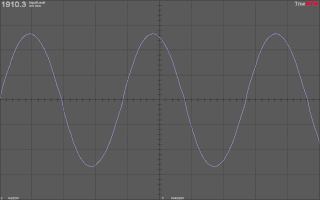
\includegraphics[scale=0.75]{aufgaben/25.png}
\end {center}

\subsubsection*{Quelltext}

\lstinputlisting[linerange=8-999,firstnumber=8,caption=aufgabe25.c]
{../MPP_WS1011/aufgaben/aufgabe25.c}

%%% Local Variables: 
%%% mode: latex
%%% TeX-master: "../Main"
%%% End: 

%%%%%%%%%%%%%%%%%%%%%%%%%%%%%%%%%%%%%%%%%%%%%%%%%%%%%%%%%%%%%%%%%%

\clearpage
\section
{\href{http://cst.mi.fu-berlin.de/intern/19606-P-MPP/Aufgaben/041000.html}
{DMA}}
%\addcontentsline{toc}{section}{DMA}

\subsection*
{\href{http://cst.mi.fu-berlin.de/intern/19606-P-MPP/Aufgaben/041001.html}
{Aufgabe 26: Der Funktionsgenerator im DMA Betrieb}}

\subsubsection*{Quelltext}

\lstinputlisting[linerange=8-999,firstnumber=8,caption=aufgabe26.c]
{../MPP_WS1011/aufgaben/aufgabe26.c}

%%%%%%%%%%%%%%%%%%%%%%%%%%%%%%%%%%%%%%%%%%%%%%%%%%%%%%%%%%%%%%%%%%

\clearpage
\section
{\href{http://cst.mi.fu-berlin.de/intern/19606-P-MPP/Aufgaben/041100.html}
{Transceiver}}
%\addcontentsline{toc}{section}{Transceiver}

\subsection
{\href{http://cst.mi.fu-berlin.de/intern/19606-P-MPP/Aufgaben/041101.html}
{Aufgabe 27: Der Empfangsmode}}

\subsubsection*{Quelltext}

\lstinputlisting[linerange=8-999,firstnumber=8,caption=aufgabe27.c]
{../MPP_WS1011/aufgaben/aufgabe27.c}

\subsection
{\href{http://cst.mi.fu-berlin.de/intern/19606-P-MPP/Aufgaben/041102.html}
{Aufgabe 28: Sensordaten per Funk übertragen}}

Um Sensordaten per Funk übertragen zu können, müssen zwei Peripherieeinheiten  genutzt werden.
Zum einen der Transciever und zum anderen der Feuchtigkeits- / Temperatursensor.
In der Funktion \texttt{sendSensors()} werden die aktuellen Sensordaten ausgelesen und per Funk übertragen.
Um nun in jede Sekunde die Daten zu senden, wird genau jene Funktion in der \textit{Interrupt Service Routine} eines zuvor konfigurierten Timers aufgerufen.

\subsubsection*{Quelltext}

\lstinputlisting[linerange=8-999,firstnumber=8,caption=aufgabe28.c]
{../MPP_WS1011/aufgaben/aufgabe28.c}

%\subsubsection*{Beschleunigungssensor}

%\lstinputlisting[caption=mma.h]
%{../MPP_WS1011/aufgaben/mma.h}

%\lstinputlisting[linerange=9-999,firstnumber=9,caption=mma.c]
%{../MPP_WS1011/aufgaben/mma.c}


%%%%%%%%%%%%%%%%%%%%%%%%%%%%%%%%%%%%%%%%%%%%%%%%%%%%%%%%%%%%%%%%%%

\clearpage
\section{Anhang}
%\addcontentsline{toc}{section}{Anhang}

\subsection{Häufig benutzte Funktionalität}

\subsubsection*{common.c}
\lstinputlisting[caption=common.h]
{../MPP_WS1011/aufgaben/common.h}
\lstinputlisting[caption=common.c]
{../MPP_WS1011/aufgaben/common.c}

\subsubsection*{project.h}
\lstinputlisting[caption=project.h]
{../MPP_WS1011/aufgaben/project.h}


%%%%%%%%%%%%%%%%%%%%%%%%%%%%%%%%%%%%%%%%%%%%%%%%%%%%%%%%%%%%%%%%%%

\clearpage
\section{\href{http://cst.mi.fu-berlin.de/intern/19606-P-MPP/Aufgaben/041200.html}
{Projekt}}
%\addcontentsline{toc}{section}{Projekt}

\subsubsection*{Idee}

Idee war die Darstellung von \href{https://secure.wikimedia.org/wikipedia/de/wiki/Lissajous-Figuren}
{Lissajous-Figuren} auf dem Oszilloskop mit Hilfe des DMA-Controllers und  des Digital-Analog-Umwandlers.

Das Bild eines Oszilloskop kann mittels zwei Spannungseingängen manipuliert werden.
Punkte werden wie in einem Koordinaten-System mittels x- und y-Werten beschrieben.
Einer der beiden Eingänge des Oszilloskops steht für den x-Wert und der andere für den y-Wert.

Ziel war es nun über zwei Digital-Analog-Umwandler jeweils bereits berechnete Sinus-Werte in analoge Spannungen umzuwandeln und mit Hilfe dieser Spannungen Figuren auf dem Oszilloskop zu zeichnen. 

Hierzu wurden bei der Initialsierung des Mikrocontrollers die komplette Periode eines Sinus vorberechnet.
Da die Werte später über den Digital-Analog-Umwandler auf dem Oszilloskop ausgegeben werden,
wurde der jeweilige Sinus-Wert noch auf einen Bereich von 0 bis 3V erhöht, sowie in eine 12 Bit Zahl konvertiert.

Der DMA-Controller ist für das Kopieren der Sinus-Werte in den jeweiligen Digital-Analog-Umwandler zuständig.
Dieser wurde so konfiguriert, dass er zuvor initialisierte Timer als Trigger benutzt und den nächstfolgenden Sinus-Wert in das Register des jeweiligen Digital-Analog-Umwandlers kopiert.

Je nach eingestellten Timer-Trigger-Werten und somit anderem Frequenzverhältnissen, können nun andere Lissajous-Figuren auf dem Oszilloskop dargestellt werden.

Bei der Umsetzung wurde auch eine eigene Bibliothek für die jeweiligen Peripherieeinheiten des Mikrocontrollers geschrieben.

\subsubsection*{Quelltext}

\lstinputlisting[caption=project.h]{../MPP_WS1011/project/project.h}

\lstinputlisting[caption=project.c]{../MPP_WS1011/project/project.c}

\subsubsection*{Bibliotheken}

\lstinputlisting[caption=adu.h]{../MPP_WS1011/project/lib/adu.h}
\lstinputlisting[caption=dac.h]{../MPP_WS1011/project/lib/dac.h}
\lstinputlisting[caption=dma.h]{../MPP_WS1011/project/lib/dma.h}
\lstinputlisting[caption=mma.h]{../MPP_WS1011/project/lib/mma.h}
\lstinputlisting[caption=timer.h]{../MPP_WS1011/project/lib/timer.h}
\lstinputlisting[caption=uart.h]{../MPP_WS1011/project/lib/uart.h}


\end{document}
